\section{Introduction}
High angular resolution
For Radio Astronomy, angular resolution is tied to the antenna dish diameter
large dishes are expensive
interferometers use several smaller antennas together
Higher angular resolution and cheaper construction.
New Radio Interferometers. like MeerKAT

Interferometers do not measure the sky in pixels. Each antenna pair measures a Fourier Component
Measure Fourier Components.
But the image reconstruction forms an ill-posed inverse problem
We have many possible images that fit the measurements.
Image reconstruction has to find the most likely image.

larger problem size require distributed computing
so far, it was difficult to separate the image reconstruction
Too much work was multiplied by the number of nodes.
Mostly done on a limited number of shared-memory systems

Target to distribute the image reconstruction
First tests


\subsection{Ill-posed inverse Problem}
The figure \ref{intro:system} shows a simplified interferometer and its whole pipeline. From Measurements to image.
Interferometer consists of several antennas
Each antenna pair forms a baseline. The signal of the two antennas get correlated, which gives us a Fourier Component. Phase and amplitude.
Its called Visibilities
Noisy measurements
Only a limited number of Visibilities. This is where the incompleteness comes in. We do not have enough data.

\begin{figure}[h]
	\centering
	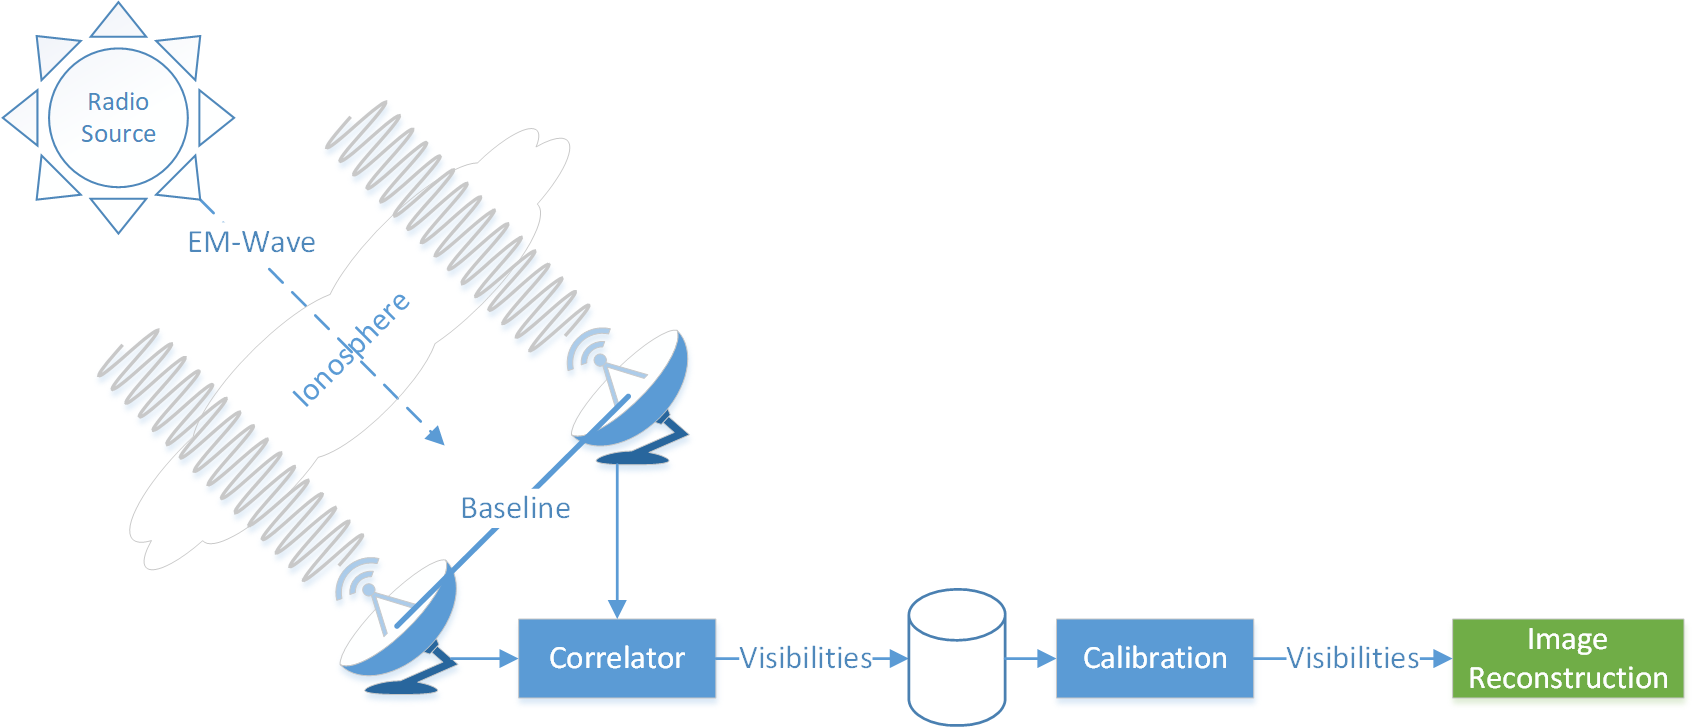
\includegraphics[width=0.80\linewidth]{./chapters/01.intro/system.png}
	\caption{Interferometer System}
	\label{intro:system}
\end{figure}

[Calibration has to be done before imaging. Large number
Then imaging is done. Imaging is the ill-posed inverse problem. Because we only have a limited number of visibilities, and because we cannot measure all 

[Calibration can be improved by using the ]

The ill-posed inverse problem still mainly comes down to the image reconstruction.


\subsection{Image Reconstruction Problem}
From the measurements, we want to reconstruct the image, which is the ill-posed inverse problem. Or more formally in equation \eqref{intro:inverseproblem}:

\begin{equation}\label{intro:inverseproblem}
V(u, v, w) = \int\int \frac{I(x, y)}{\sqrt{1 - x^2 - y ^2}} e^{2 \pi i [ux+vy+ w(\sqrt{1 - x^2 - y ^2} - 1)]} \: dx \: dy
\end{equation}

We try to find the image $I()$, while we only have the Visibilitiy measurements $V()$
Three dimensional Visibility space.
Furthermore, $V()$ is noisy.

An example is shown in figure \ref{intro:inversefig}.

\begin{figure}[htp]
	% preliminary
	\sbox\twosubbox{%
		\resizebox{\dimexpr.9\textwidth-1em}{!}{%
			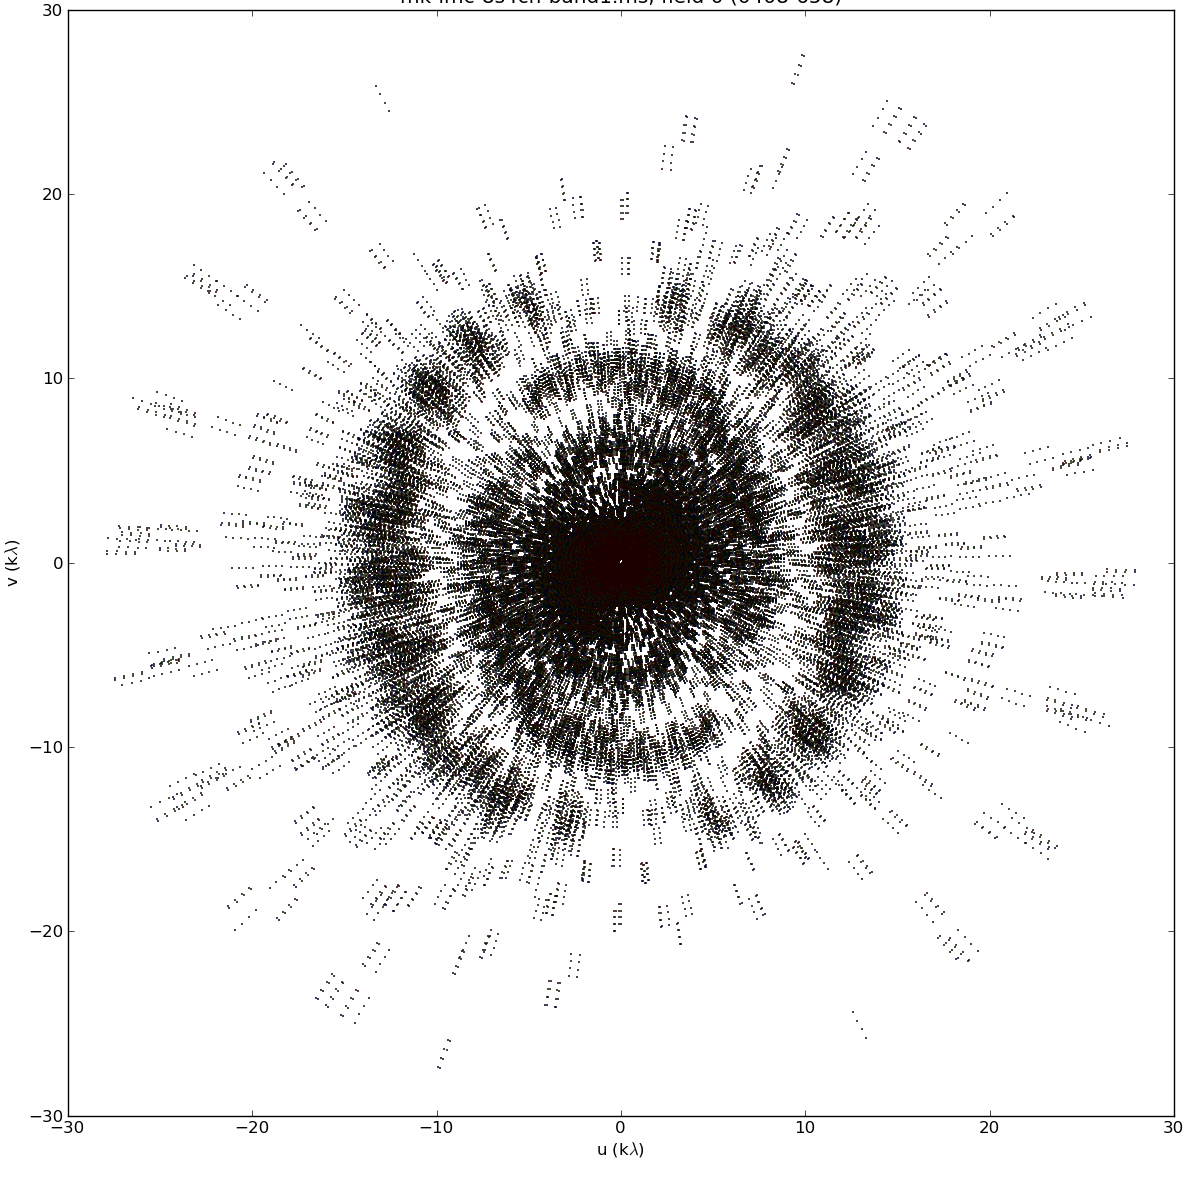
\includegraphics[height=3cm]{./chapters/01.intro/meerkat_uv2.png}%
			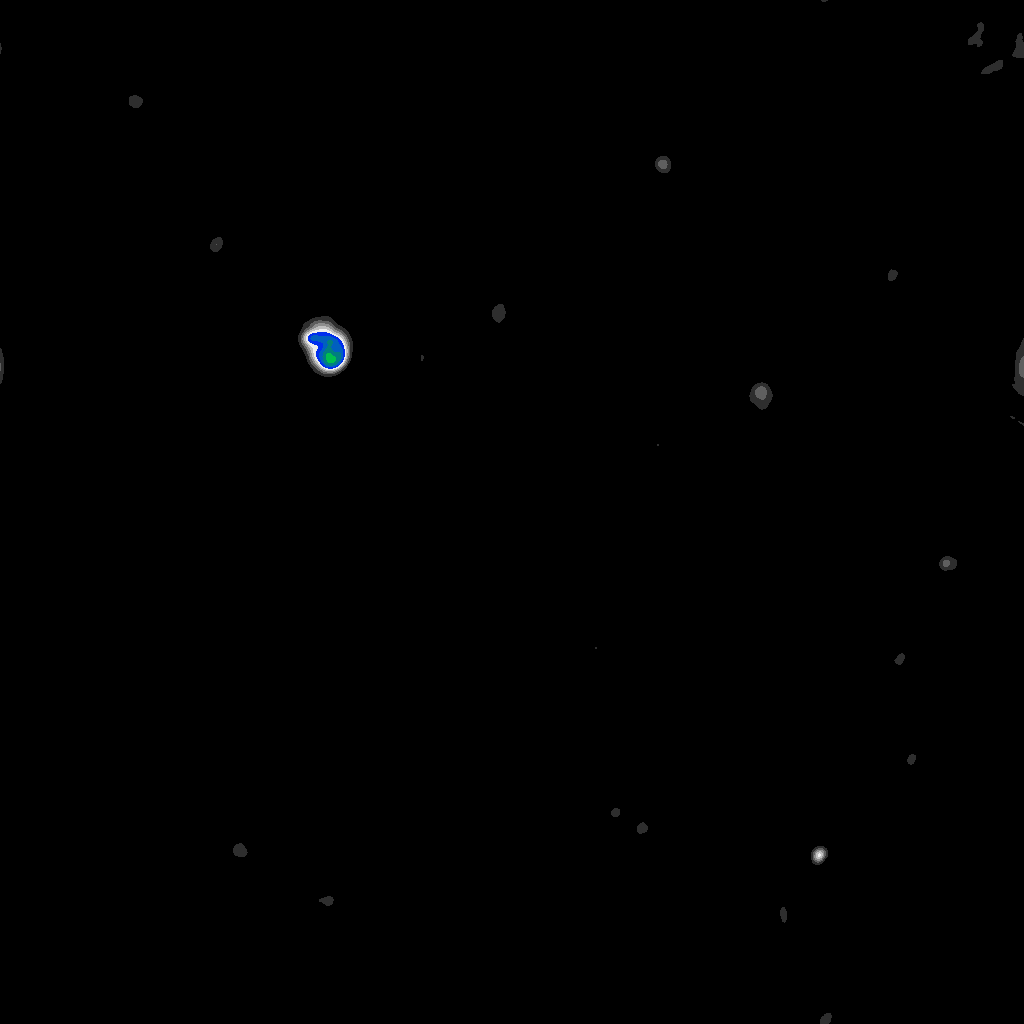
\includegraphics[height=3cm]{./chapters/01.intro/mk2/clean.png}%
		}%
	}
	\setlength{\twosubht}{\ht\twosubbox}
	
	% typeset
	\centering
	\subcaptionbox{Measurements $V()$ in the UV plane.\label{intro:inversefig:uvspace}}{%
		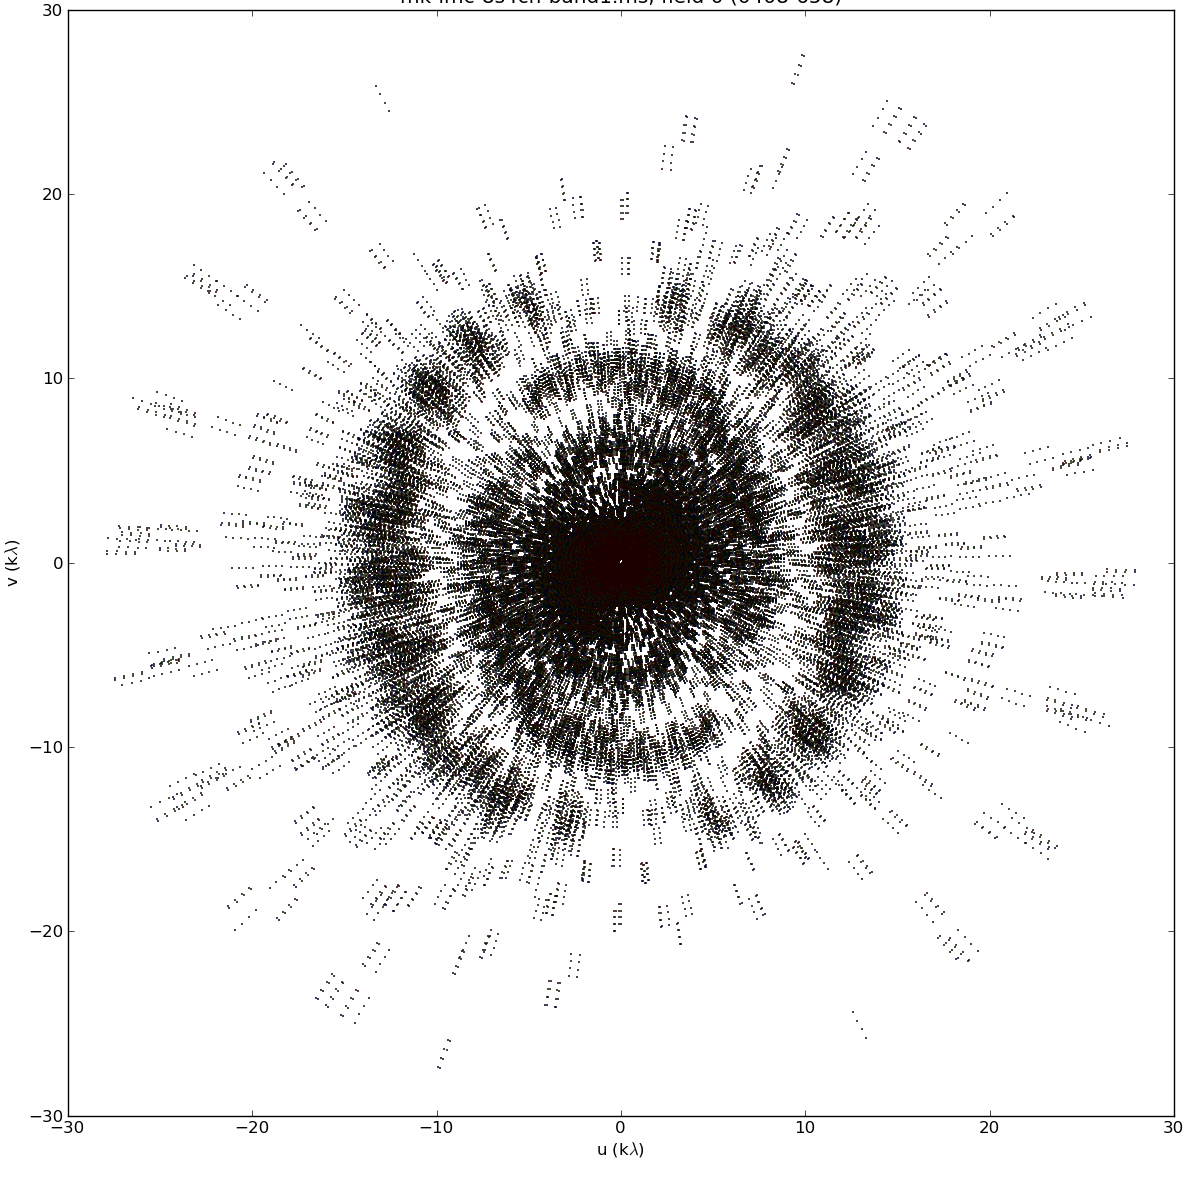
\includegraphics[height=\twosubht]{./chapters/01.intro/meerkat_uv2.png}%
	}\quad
	\subcaptionbox{A reconstructed image $I()$ which fits the measurements.\label{intro:inversefig:reconstruction}}{%
		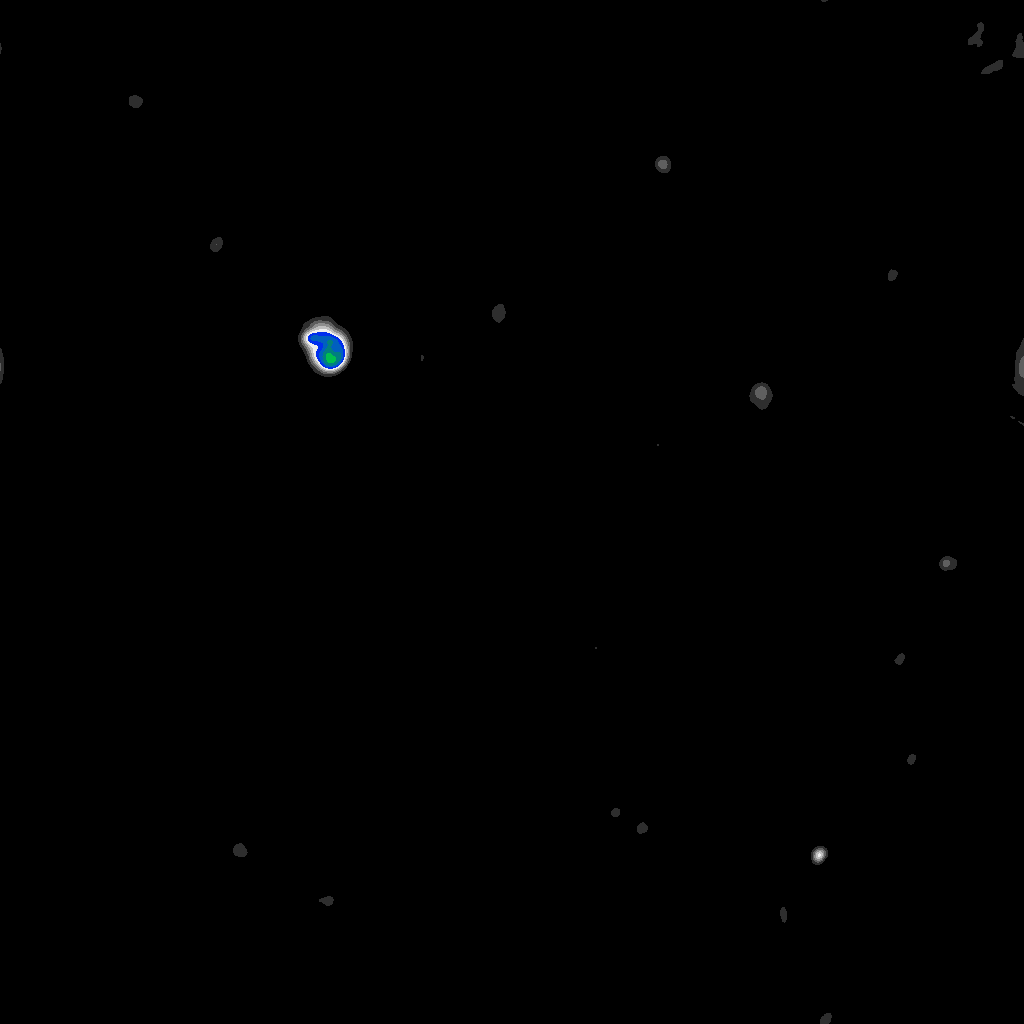
\includegraphics[height=\twosubht]{./chapters/01.intro/mk2/clean.png}%
	}
	\caption{The Image Reconstruction Problem}\label{intro:inversefig}
\end{figure}



\subsubsection{Representing the reconstruction problem}


